\section{Evaluation}\label{sec:eval}

\begin{figure*}[t]
  \centering
  \begin{subfigure}[t]{0.48\textwidth}
    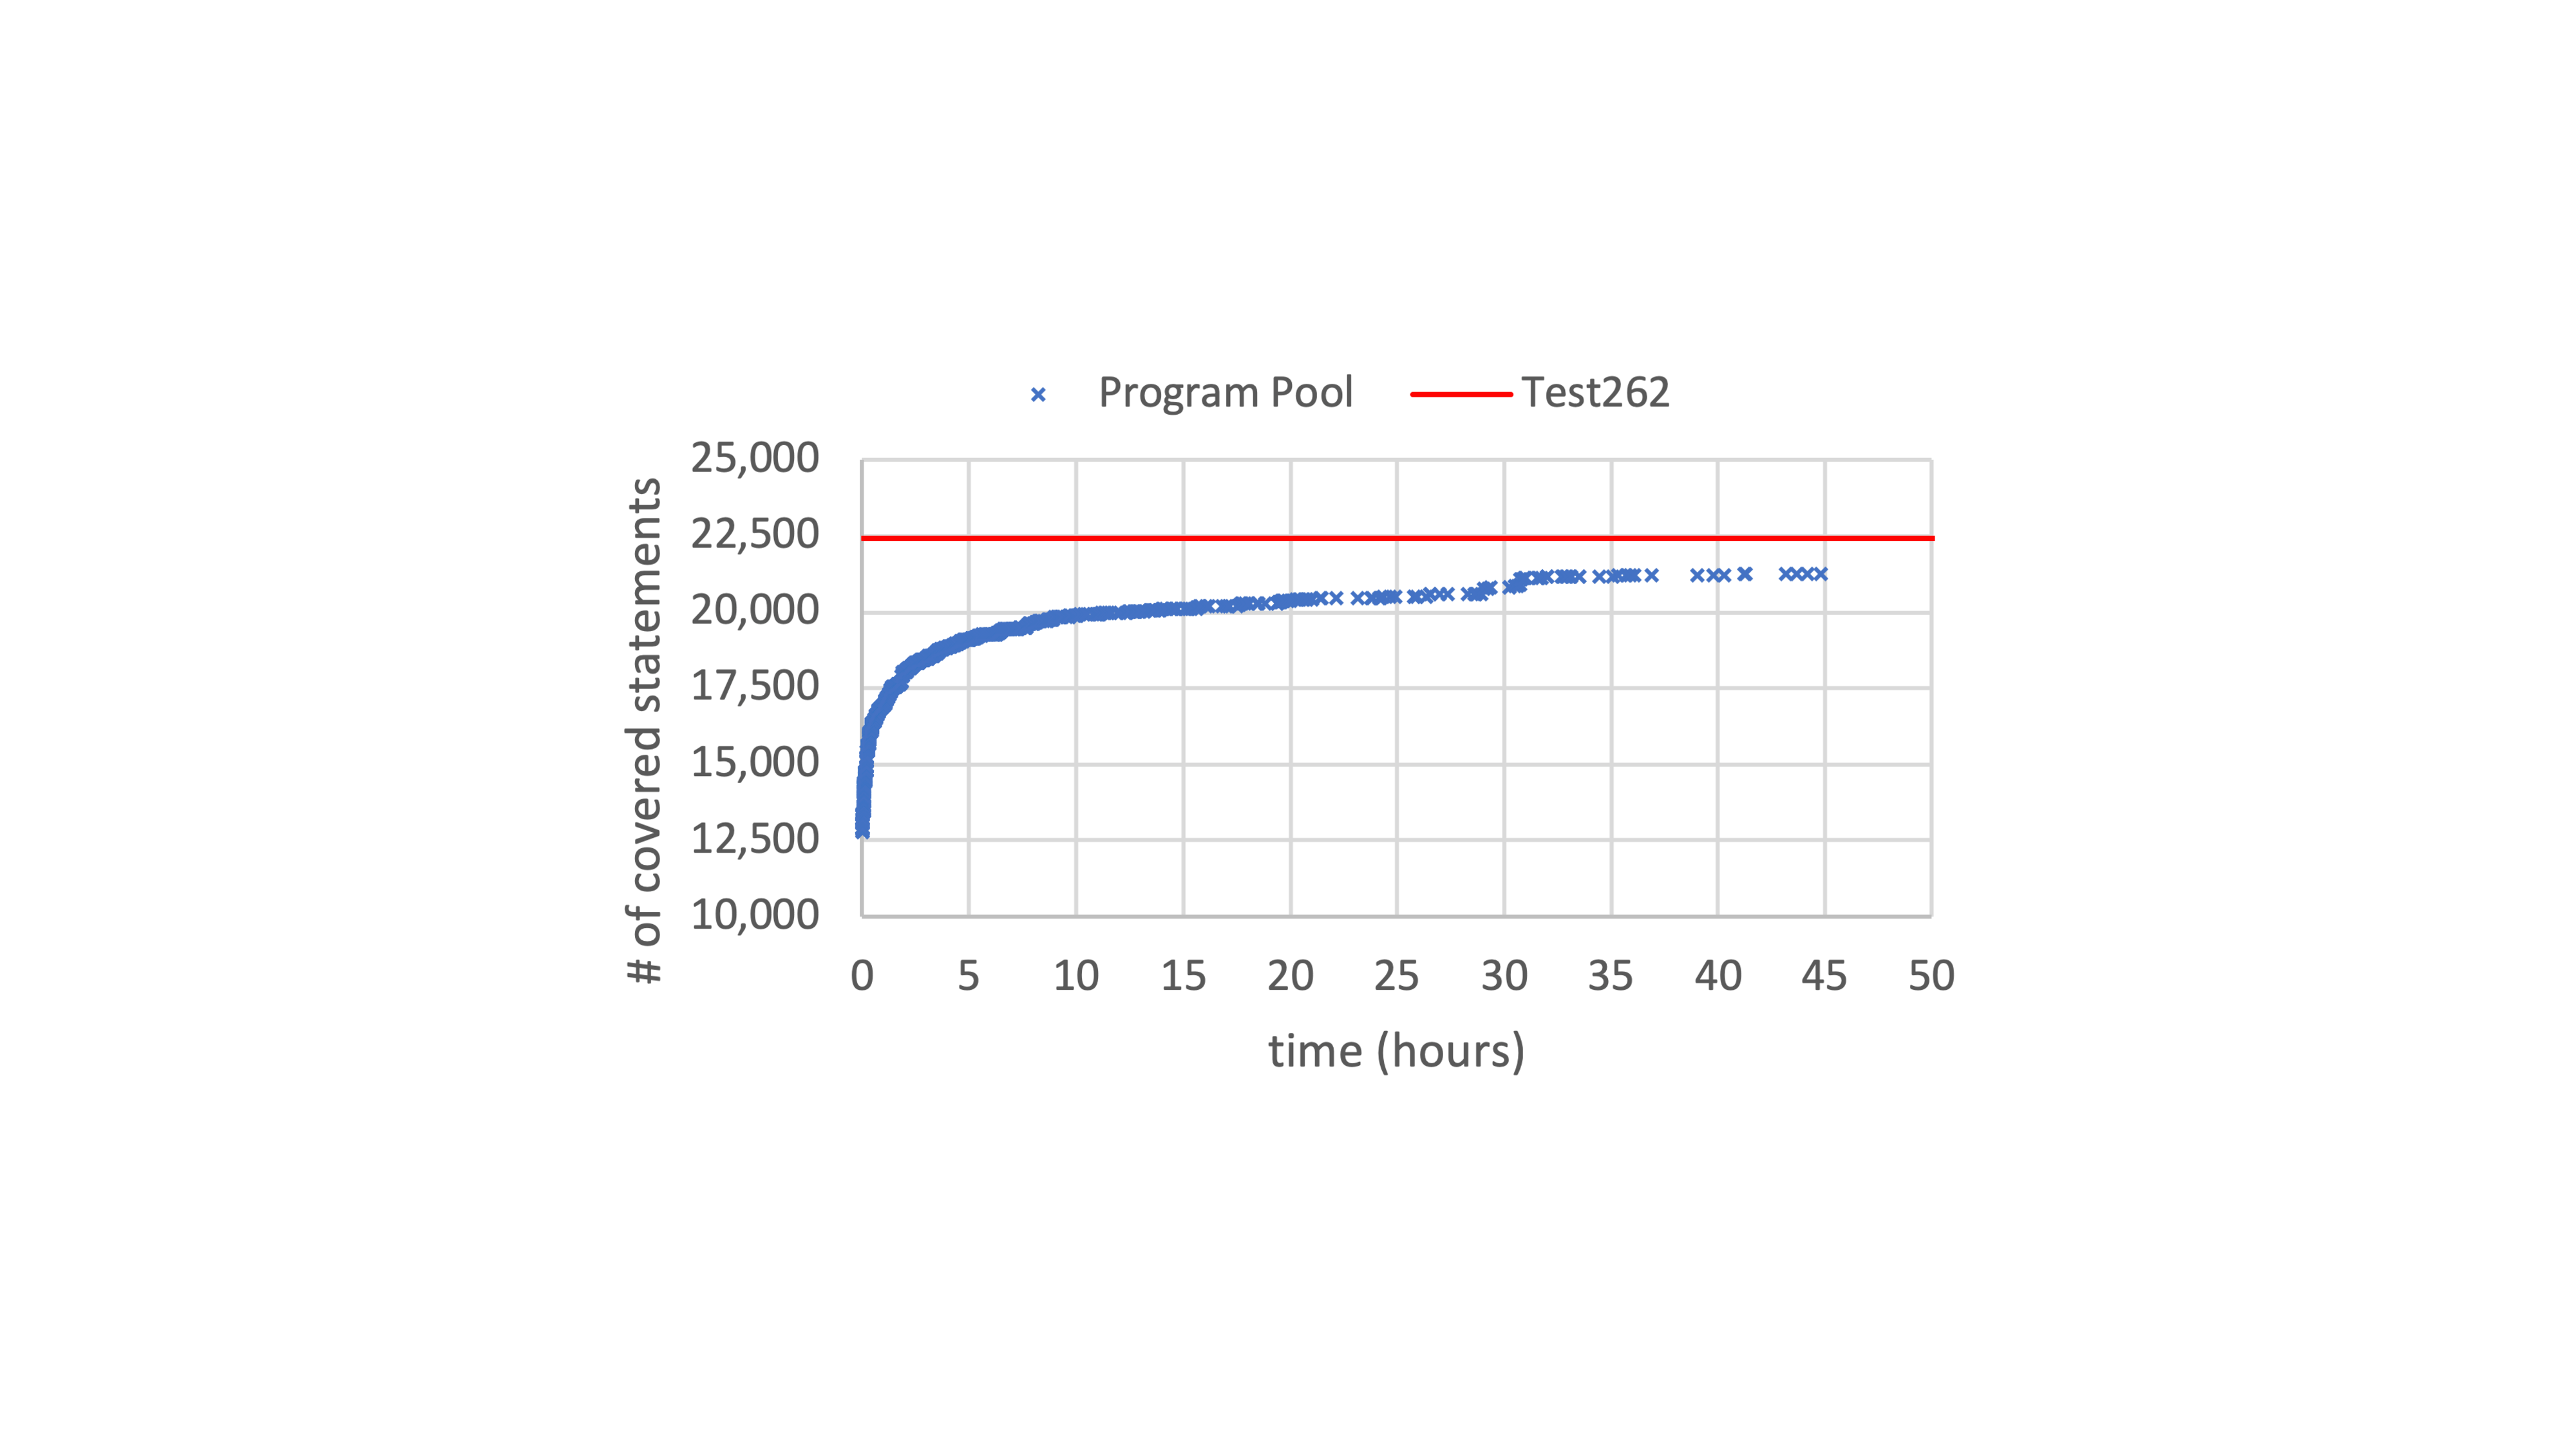
\includegraphics[width=\textwidth]{img/stmt-coverage.pdf}
    \caption{The statement coverage}
    \label{fig:stmt-coverage}
  \end{subfigure}
  \quad
  \begin{subfigure}[t]{0.48\textwidth}
    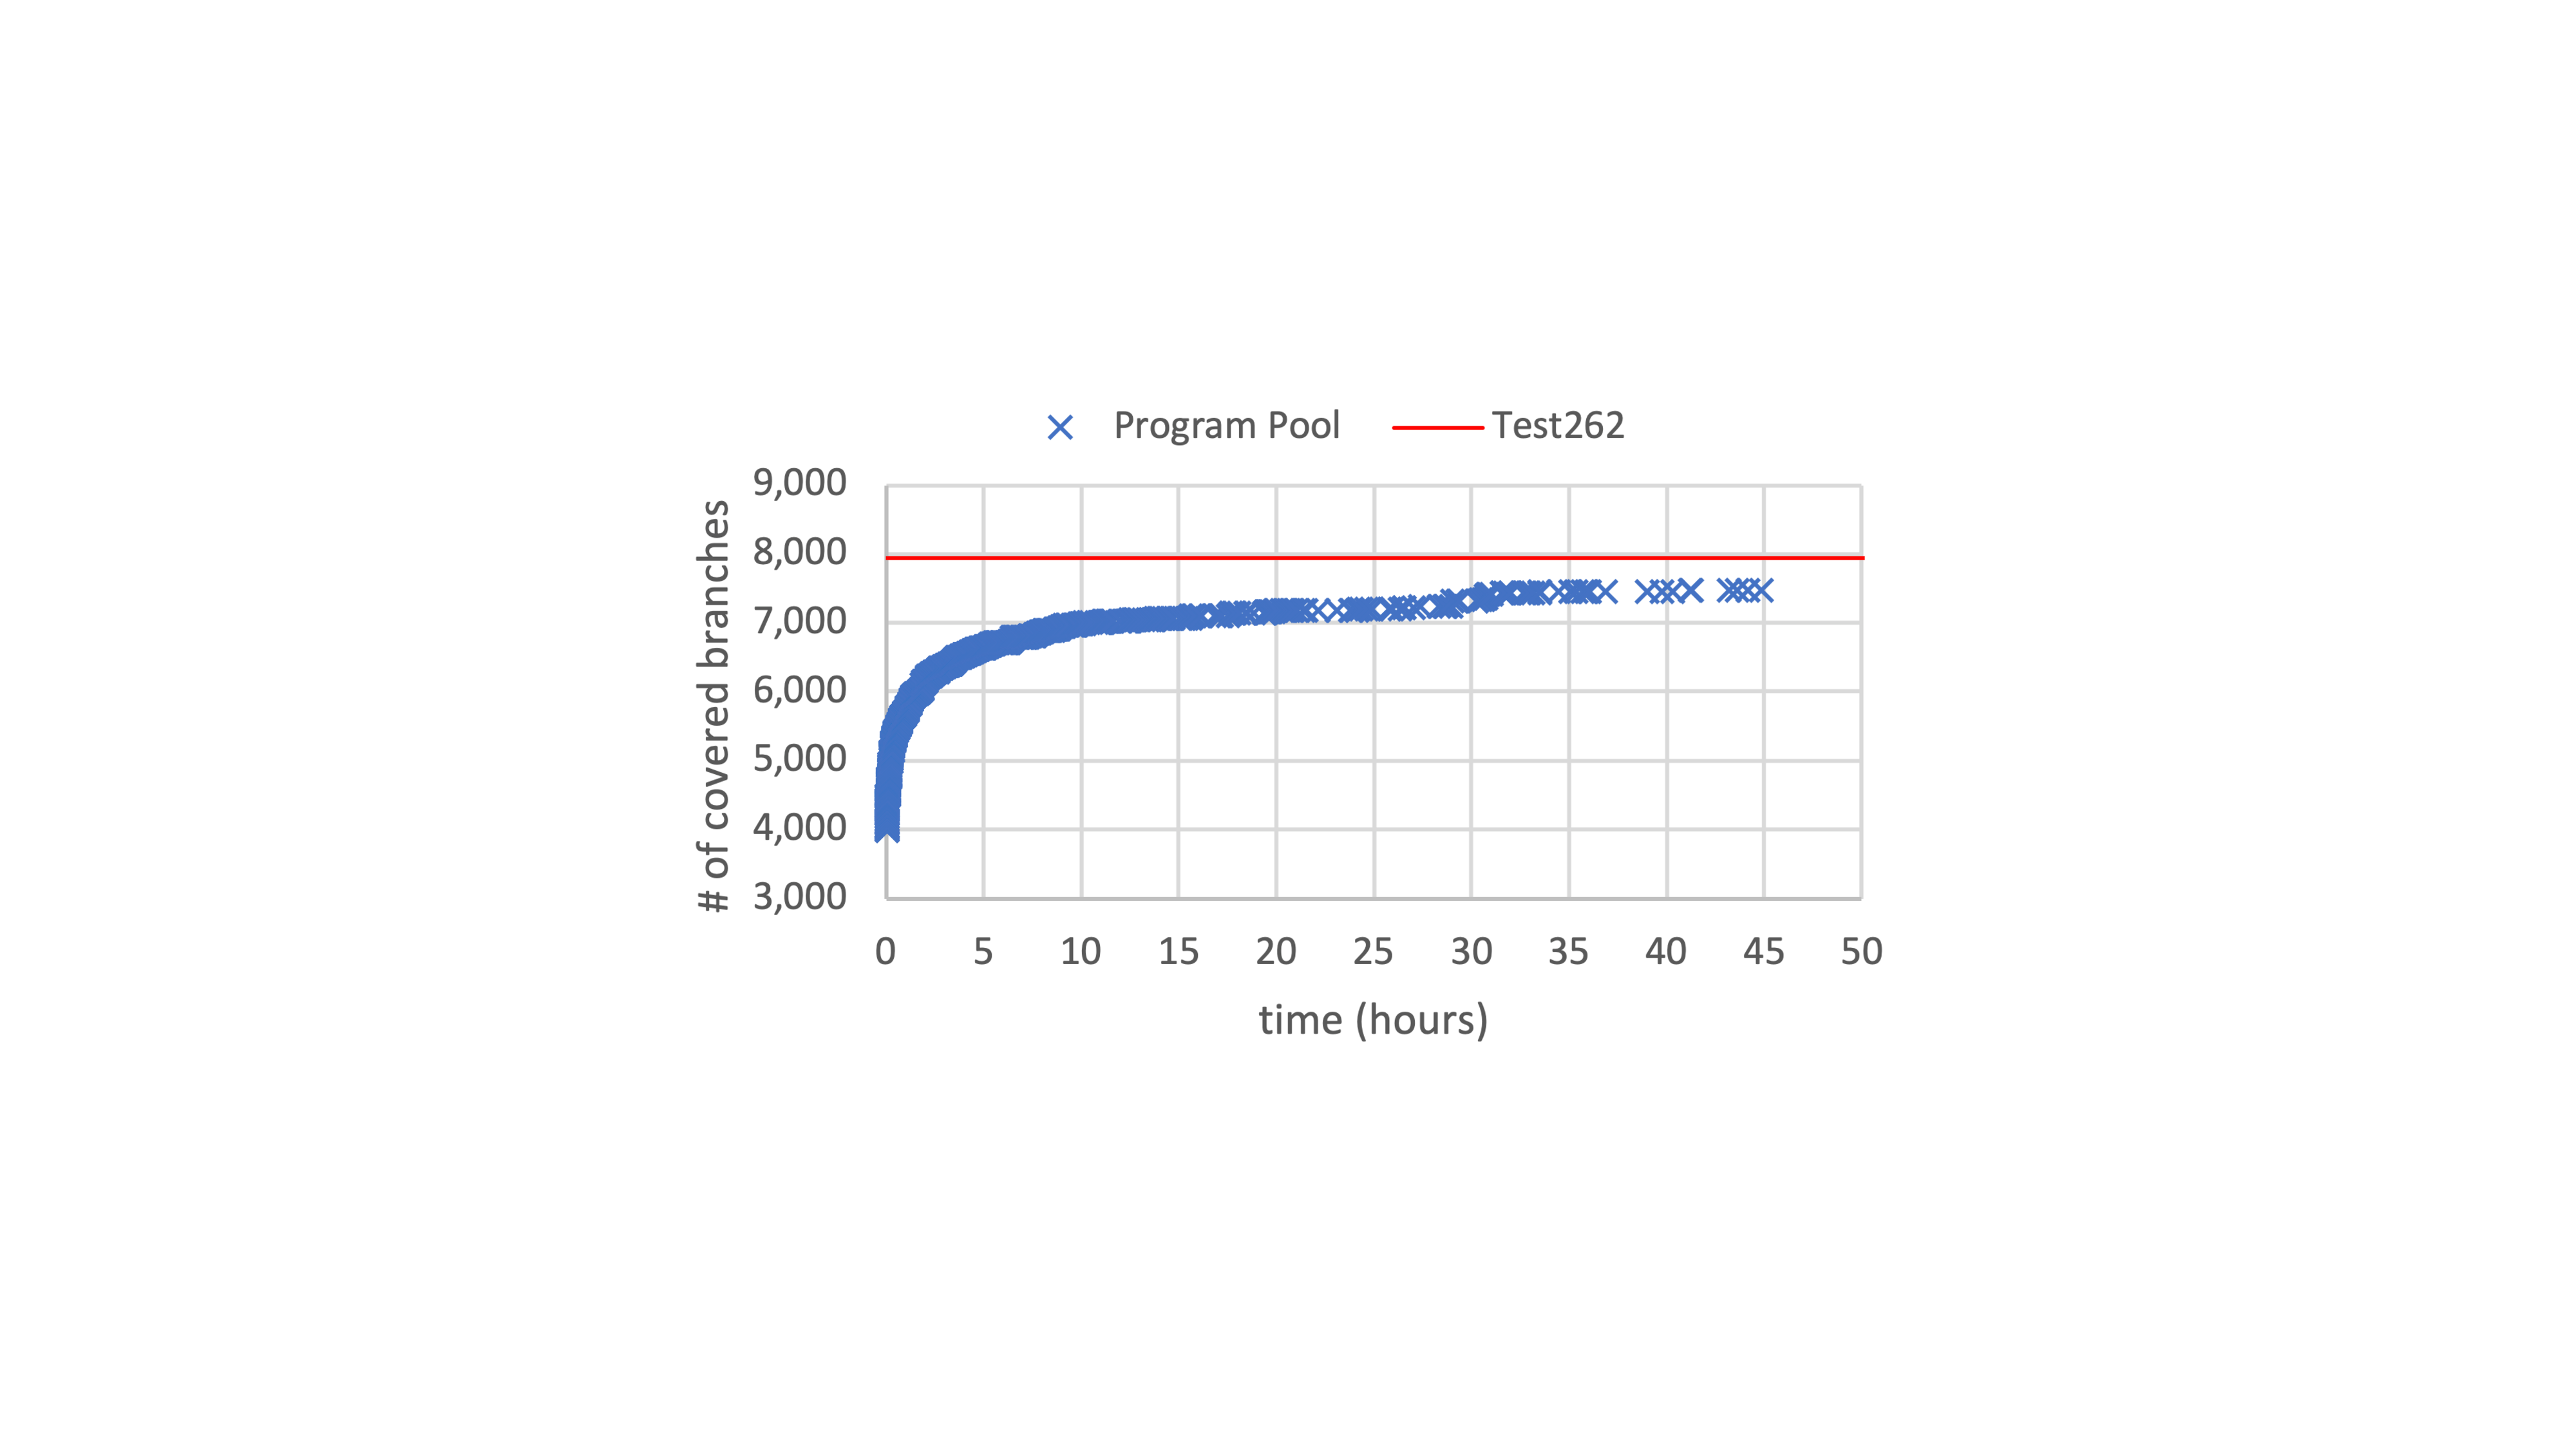
\includegraphics[width=\textwidth]{img/branch-coverage.pdf}
    \caption{The branch coverage}
    \label{fig:branch-coverage}
  \end{subfigure}
  \caption{The semantics coverage changes during the test generation phase}
  \label{fig:sem-coverage}
  \vspace*{-1em}
\end{figure*}

To evaluate $\tool$ that performs the $N$+1-differential testing of JavaScript
engines and specification, we applied our tool to four JavaScript engines that
fully support modern JavaScript features and the most recent specification,
ECMAScript 2020 (ES11, 2020).  We targeted the following four JavaScript
engines and all of them supports
ES11\footnote{https://github.com/graalvm/graaljs\#current-status}\footnote{https://bellard.org/quickjs/}\footnote{https://blog.moddable.com/blog/xs10/}\footnote{https://v8.dev/}:
\begin{itemize}
  \item \textbf{GraalJS(v20.1.0):} A JavaScript implementation built on
    GraalVM\cite{graaljs}, which is a Java Virtual Machine (JVM) based on
    HotSpot/OpenJDK developed by Oracle.
  \item \textbf{QuickJS(2020-04-12):} A small and embedded JavaScript engine developed by
    Fabrice Bellard and Charlie Gordon\cite{qjs}.
  \item \textbf{Moddable XS(v10.2.1):} A JavaScript engine at the center of the Moddable
    SDK\cite{xs}, which is a combination of development tools and runtime
    software to create applications for microcontrollers.
  \item \textbf{V8(v8.5):} The Google's open source high-performance JavaScript and
    WebAssembly engine\cite{v8}, written in C++.
\end{itemize}
To extract mechanized specification from ECMAScript, we utilize the tool
$\jiset$, which is a JavaScript IR-based semantics extraction toolchain.
automatically extracted from a given ECMAScript.  We performed our experiments
on a machine equipped with 4.0GHz Intel(R) Core(TM) i7-6700k and 32GB of RAM
(Samsung DDR4 2133MHz 8GB*4).  We evaluated our tool based on the following four
research questions:
\begin{itemize}
  \item {\bf RQ1 (Coverage of Generated Tests)} The semantics coverage compared
    to Test262, the official conformance test suite for ECMAScript.
  \item {\bf RQ2 (Bug Detection in JavaScript Engines)} The number of bugs in
    four JavaScript engines detected by $\tool$.
  \item {\bf RQ3 (Bug Detection in ECMAScript)} The number of specification bugs
    in ES11 detected by $\tool$.
\end{itemize}


\subsection{Coverage of Generated Tests}

For the first step, we synthesize seed programs via \textsf{Seed Synthesizer}
based on the syntax of ES11.  It synthesizes \inred{1,112} JavaScript programs
in about \inred{10} seconds and covers \inred{97.25\% (395/406)} of reachable
alternatives in syntax productions.  The seed programs becomes the initial
program pool and it gradually grows via \textsf{Target Selector} and
\textsf{Program Mutator}.  Figure~\ref{fig:sem-coverage} shows the change of
semantics coverage of the program pool during the iterative process in
\inred{45} hours.  The left and right graphs show the statement and branch
coverages, respectively.  The red line for each graph denotes the coverage of
tests of Test262.  For the statement coverage, \inred{29,728} statements exist
in ES11 and tests in Test262 covers \inred{22,425 (75.43\%)} statements.  The
initial program pool covers \inred{12,766 (42.94\%)} statements and the final
program pool covers \inred{21,249 (71.48\%)} statements.  For branch coverage,
\inred{11,448} branches exist in ES11 and tests in Test262 covers \inred{7,944
(69.39\%)} branches.  The initial program pool covers \inred{3,986 (34.82\%)}
branches and the final program pool covers \inred{7,476 (65.30\%)} branches.

\begin{table}
  \caption{The number of successes and covered branches for mutation methods}
  \label{table:mutation-method}
  \vspace*{-1em}
  \small
  \[
    \begin{array}{l|r|r}
      \telembf{c|}{Mutation Methods}      & \telembf{c|}{Success}& \telembf{c}{Branch (Avg.)}\\\hline
      \text{Nearest Syntax Tree Mutation} & \rtext{436}       & \rtext{1,450 (3.33)}\\\hline
      \text{Random Mutation}              & \rtext{320}       & \rtext{910   (2.84)}\\\hline
      \text{Statement Insertion}          & \rtext{201}       & \rtext{672   (3.34)}\\\hline
      \text{Object Substitution}          & \rtext{162}       & \rtext{453   (2.80)}\\\hline
      \text{String Substitution}          & \rtext{4}         & \rtext{5     (1.25)}\\\hline
      \hline
      \telembf{c|}{Total}                 & \rtext{1,123}     & \rtext{3,490 (3.11)}\\
    \end{array}
  \]
  \vspace*{-1.5em}
\end{table}

Table~\ref{table:mutation-method} shows the number of successes and covered
branches for each mutation method during the test generation phase. In total,
$\tool$ succeeds to synthesize \inred{1,123} programs that covers \inred{3,490}
more branches than the initial program pool.  Among five mutation methods, the
nearest syntax tree mutation is the most contributed method (\inred{436}
successes and \inred{1,450} covered branches) and the least one is the string
substitution (\inred{4} successes and \inred{5} covered branches).  On average,
\inred{3.11} branches are covered by one successful mutation.


\subsection{Bug Detection in JavaScript Engines}
\inred{TODO}


\subsection{Bug Detection in ECMAScript}
\inred{TODO}
